\chapter{Cosmic rays}
\label{ch:cosmic-rays}


\section{History of cosmic-ray research}

Cosmic rays were not discovered over night, the discovery extends over a century. In 1785 their effects were detected by de Coulomb \cite{coulomb1785electroscope} [alternative, in english] with an electroscope. An electroscope measures the amount of electrical charge in a test object. De Coulomb saw it unexpectedly discharge in the air, even though it was properly insulated.

In fact the effects of low-energy solar cosmic rays were seen much earlier, in the form of the aurora borealis and aurora australis. Named such in the 17th century. Several ancient written recordings of the phenomenon \cite{stephenson2004aurora} have been found, moreover, many folk tales about this phenomenon exist. The aurora is caused by disturbances in the magnetosphere of the Earth. The disturbances are generally caused by solar winds. The disturbances cause charged particles to be accelerated along the magnetic field lines into the atmosphere. There the particles will excite and ionize oxygen and nitrogen atoms. When these de-excite or recombine the observed colors are produced. An example of the aurora can be seen in \cref{fig:aurora}.

In 1895 the discovery of X-rays and their capability to ionize air \cite{roentgen1895radiation,flakus1981radiation} presented a good candidate for the discharge of the electroscope. However, a source of the X-rays had not yet been identified. In 1896 Becquerel discovered the existence of radioactivity. he also found that the radiation from radioactive material couple cause an electroscope to discharge. In 1600 Gilbert created a terrela, a sphere with a magnetic field resembling that of the Earth \cite{gilbert1893terrela-en}. In 1896 Birkeland \cite{birkeland1896aurora} showed that electron beams fired at a terrela were bent along the field lines to form circular regions around the magnetic poles like the aurora. Further experiments with the electroscopes were performed to assertain the source of the ionizing radiation. Experiments went over seas, underwater, underground, and far above ground (Eiffel Tower), but no conclusive evidence for cosmic rays was found until Hess performed balloon flights in 1911 and 1912 which accurately determined the amount of radiation at various altitudes. It showed a clear increase at very high altitudes, indicating an extra-terrestial source for the radiation. Clay found that the intensity of the ionization depended on latitude. This latitudinal dependency could be caused by the magnatic field of the Earth. Begin affected by magnetic fields indicates that the particles were charged particles. The indepent discovery of extensive air showers (EAS) by Auger (1939) \cite{auger1939eas} and Rossi (1934) ignited the cosmic-ray research field. New possibilities for studying cosmic rays were found.

\begin{figure}
    \centering
    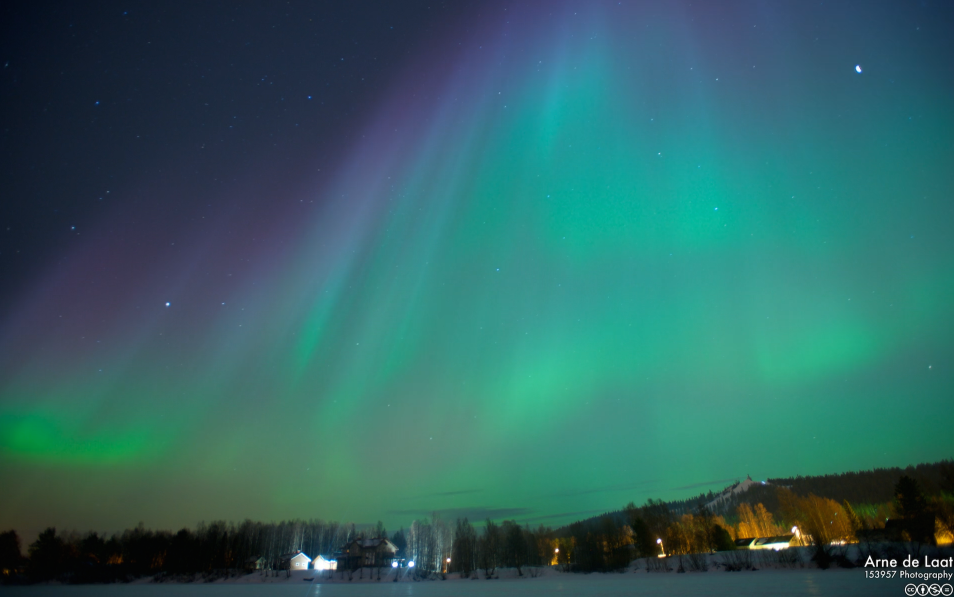
\includegraphics[width=0.6\textwidth]{plots/cosmic-rays/aurora.png}
    \caption{The aurora borealis as seen in Rovanemi, Finland on 17 March 2015, St. Patricks day. The large aurora activity on that day was due to a G4 geomagnetic storm on the sun on the 15th.}
    \label{fig:aurora}
\end{figure}


\subsection{Balloon and space experiments}

Other experiments also took to the sky because that is where the cosmic rays could be detected before they underwent collisions with particles in the atmosphere. Ground-based experiments only see the remnants of the EAS. Being able to directly detect the particle has many advantages. Such as better energy and direction resolution, and easier particle identification.

The main downside is the flux of cosmic-rays decreases steeply when looking at higher-energy cosmic rays. Ideally you would have a detector with a large detection area and a very long exposure time. Unfortunately a detector that has to be flown at the top of the atmosphere or in space can only be so big before it costs too much to launch. Balloon experiments are often short runs where the balloon carrying the detector stays up for about a week. The JACEE \cite{asakimori1998jacee} and RUNJOB \cite{hareyama2011runjob} experiments flew multiple times. Each experiment reached a total fly time of \SI{60}{\day}. Notable space-based missions are PAMELA \cite{adriani2014pamela}, in orbit on the Resurs DK1 sattelite since 2006, and the AMS-02 \cite{casaus2014ams} experiment attached to the ISS since 2011. These space-based experiments have been operating for many years providing good resolution on the composition of cosmic rays at energies below the knee \cite{kulikov1958knee}. The longest running space-based cosmic-ray experiments are the Voyager spacecrafts. The Voyager spacecrafts were launched in 1977 to use the planetary alignment to accellerate with several gravity assists [ref Stone]. In August 2011 Voyager I seems to have reached the heliopause of the solar system, at \SI{121}{\astronomicalunit} distance to the Sun. Here the detection rate of particles caused by the solar wind (>\SI{0.5}{\MeV}) decreased steeply and the rate of cosmic-ray particles from outside the solar system (>\SI{70}{\MeV}) increased significantly (see figure/ref). These particles are thought to originate from supernovae in this galaxy.

There have been many more of experiments of this type, all together providing a very detailed picture of the low energy cosmic-ray spectrum. The per-nucleus spectrum of such experiments is shown in \cref{fig:low_e_spectrum}.

\begin{figure}
    \centering
    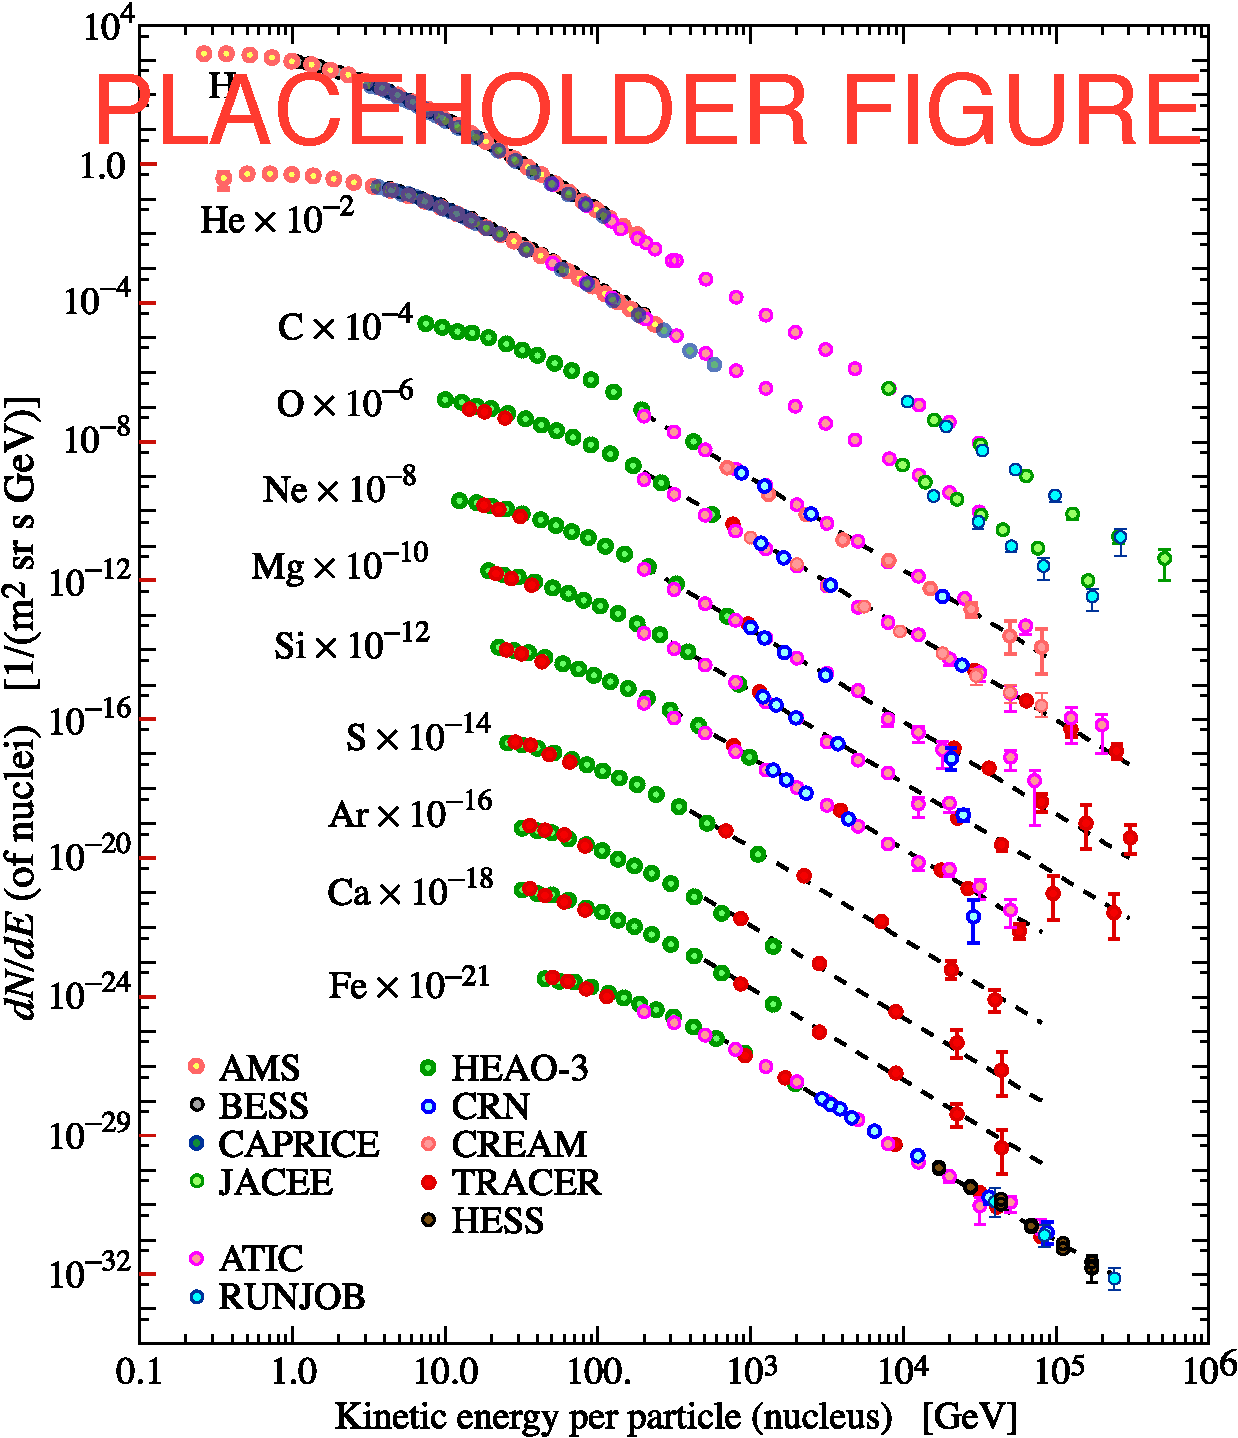
\includegraphics[width=0.6\textwidth]
                    {plots/cosmic-rays/PDG_28_1_fluxes_per_nucleus}
    \caption{Per nucleus spectrum of cosmic-rays, reproduced from \cite{olive2014pdg}.}
    \label{fig:low_e_spectrum}
\end{figure}


\subsection{Ground-based experiments}

In the previous section the difficulty of direct measurements of high energetic cosmic rays is emphasized. The nature of EAS, many collisions in which particles scatter, means that their showers are detectable over large distances on the ground. It is cheaper to build and operate such an experiment over a large period of time than a space-based experiment. Different experiments have focused on different aspects of air showers. Most detect EAS by detecting the leptons that arrive on the ground. Some designed for the highest energy showers, others for filling in the intermediate range. Others try to sample the shower front as accurately as possible by tightly spacing the detectors. Several experiments look at the shower development in the atmosphere by looking at the fluorescence created by the shower. In recent years radio detection of air showers has been developed. These look for a signature signal created in radio, caused by Earth's magneticfield directing the electrons and positrons in opposite directions.

Some detector arrays are situated high above sea-level with less atmosphere above the detectors and thereby closer to Xmax. This has the advantage that less extinction and scattering has occurred in the EAS, providing a cleaner look at the air shower. After Xmax particle extinction becomes dominant versus new particle creation.

Notable ground-based experiments are AGASA, KASCADE-Grande, Auger Observatory, TA, Tibet, Fly's Eye, Havanah Park, Volcano Ranch, HiRes, IceTop, CASA-MIA, Tien-Shan, Ahemo, MGU, Grigorov, Rossi/Zatsepin and other early experiments..

\begin{figure}
    \centering
    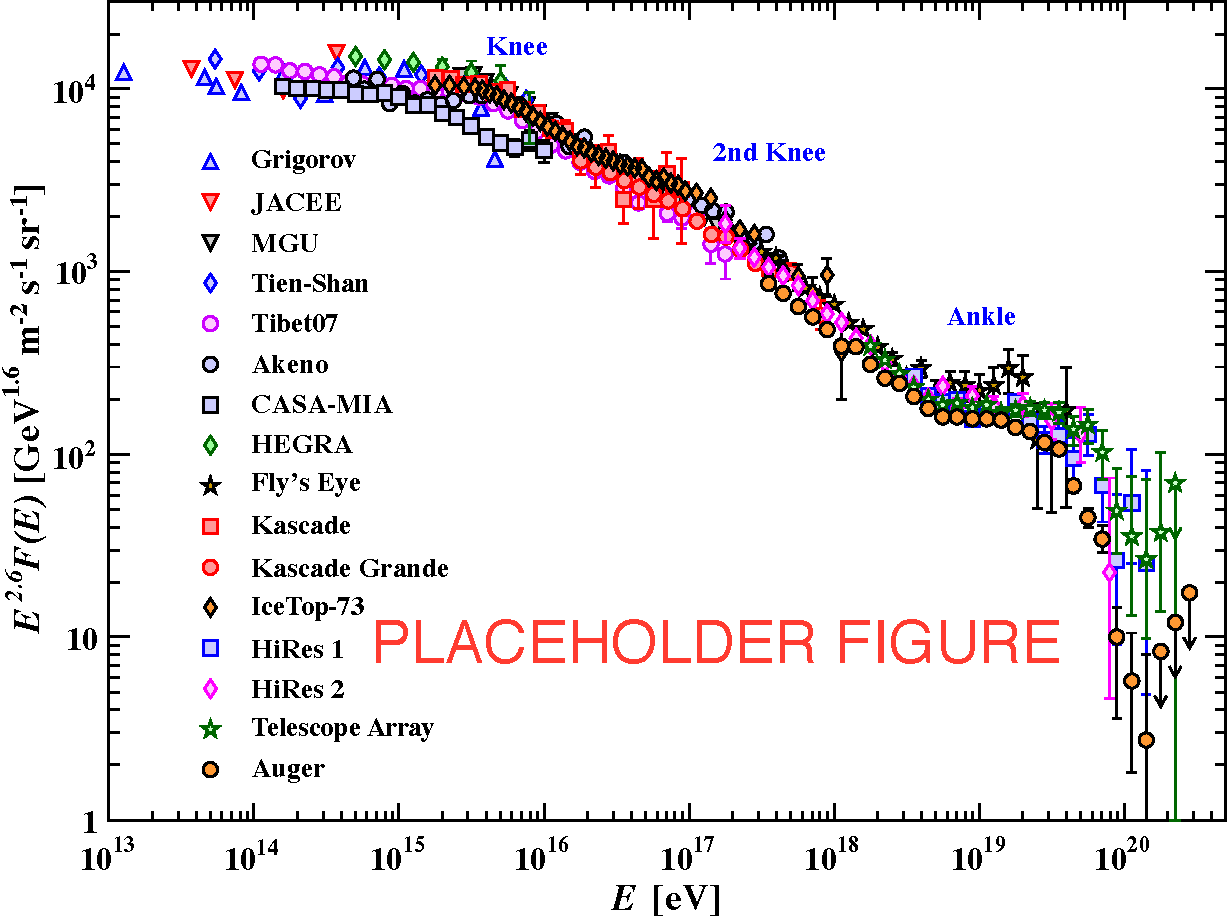
\includegraphics[width=0.6\textwidth]
                    {plots/cosmic-rays/PDG_28_8_all_particle_spectrum}
    \caption{The all particle spectrum of cosmic-rays, reproduced from \cite{olive2014pdg}.}
    \label{fig:spectrum}
\end{figure}


\section{Air-shower physics}
\label{sec:air-shower-physics}

\subsection{Shower development}

Main process, production channels. hadronic, pions, electromagnetic, muons..
Energy transfer from hadronic to electromagnetic


\subsection{Shower front}

The shower front is defined as the particle showers that pass a given surface. Particles will pass this at different distances to the shower axis (original trajectory of the primary particle). The distribution of the particles in the lateral direction is an important measure for the energy of the shower.

[figure of a shower front]

Possibly some particles later than expected, being investigated by LiO's.


\section{Air-shower simulations}

The direct cosmic-ray measurement methods are only able to effectively measure cosmic-rays up to \SI{e14}{\eV}. Particle colliders like HERA, RHIC, and SPS [refs, or see figure] have been able to produce collisions in that energy region, with equivalent center mass energies of several hunderds \si{\GeV}. However, primary cosmic rays with less than \SI{e14}{\eV} produce few particles that reach the ground. With close enough detector spacing such showers can be detected.

For ground-based detectors, the collider data has been essential for tuning models for the higher-energy collisions. Using extrapolations models can simulate the expected showers for cosmic-rays of the highest energies. The expected accuracy of the extrapolations becomes less the further they are from the collider data. These colliders provide important data about the hadron production processes in air showers, the cross-sections of the collisions, the multiplicity of secondary high-energy particles and the ratio of neutral to charged particles \cite{pierog2008lhc}.

Fermilab's Tevatron was capable of proton collisions with center of mass energies of \SI{1.8}{\TeV} \cite{abe1994tevatron}, equivalent to collisions of cosmic protons with \SI{2e15}{\eV} against a fixed target. This is approximately the lower energy limit for the KASCADE experiment. However, KASCADE's upper limit was \SI{e17}{\eV}. The LHC is in an interesting energy range; \SI{7}{\TeV} and now upgraded to \SI{14}{\TeV}, equivalent to \SI{2e16}{\eV} and \SI{e17}{\eV} cosmic-ray energies respectively. These are the first time that we have access in colliders to collision energies above the knee in the cosmic-ray spectrum. This also covers the entire energy range of the KASCADE experiment (not KASCADE-Grande). It has been shown that the hadronic interaction models did not match the new LHC data at energies beyond the Tevatron. Mismatches at slightly higher energies become big errors at very high energy. The EPOS and QGSJETII models have been updated with LHC data from the \SI{7}{\TeV} run, which should provide more accurate results for higher energies. The \SI{14}{\TeV} run of the LHC has since started, but EAS simulations used for this thesis were performed before data from that run had been incorporated into the models.

The TOTEM and LHCf experiments at the LHC are placed at the forward regions of the CMS and ATLAS interaction points respectively. These provide the most interessing data for cosmic-ray physics because the interesting products of collisions are those with high pseudorapidity. The LHC runs with p-p collisions most of the time, short periods are run with heavy ions collisions (p-Pb and Pb-Pb). However, for cosmic-ray physics collisions with low-mass ions that are commonly part of the interactions of EAS would be more interesting. Most first interactions are with oxygen, nitrogen, or argon atoms [ref, corsika?]. Collision data of such interactions would greatly benefit the cosmic-ray community.


\section{\hisparc for outreach and research}

The \textbf{Hi}gh \textbf{S}chool \textbf{P}roject on \textbf{A}strophysics \textbf{R}esearch and \textbf{C}osmics (\hisparc) is a ground-based detector experiment. It is not solely intended as an advanced cosmic-ray research experiment, but also as an outreach project which engages high-school students. Most of the \hisparc detector stations are situated at high schools, and have been built by groups of students from those schools. The building of the detectors takes several days and is done by groups of up to eight students. Because some specialized equipment is required for the construction and to properly supervise the process this is performed at a participating university.

On the first day they are introduced to cosmic-ray physics and assemble the scintillator and light-guide parts of the detector which involves glueing. This glue needs to dry for several days after which the students come again to wrap the detector to make it light tight, as can be seen in \cref{fig:detector-bouw}. Finally the photo multiplier is attached and the detector is tested in the lab before it is placed on the school roof.

Students taking physics classes are also encouraged to do their research project on \hisparc. In Dutch this project is called `profielwerkstuk' which is a mandatory part of their final year in high school. This project should be related to a subject they have chosen as their set of subjects. In order to assist these students and others that want to work with on cosmic-ray research all data recorded by \hisparc is freely available (licensed under Creative Commons BY-SA 4.0) for use. Moreover, tools are provided to assist in data analysis. On several occasions a symposium was held in which students could present their profielwerkstuk and win a trip to Cern. The subject of their project had to be about a physics field relevant for cosmic rays.

\begin{figure}
    \centering
    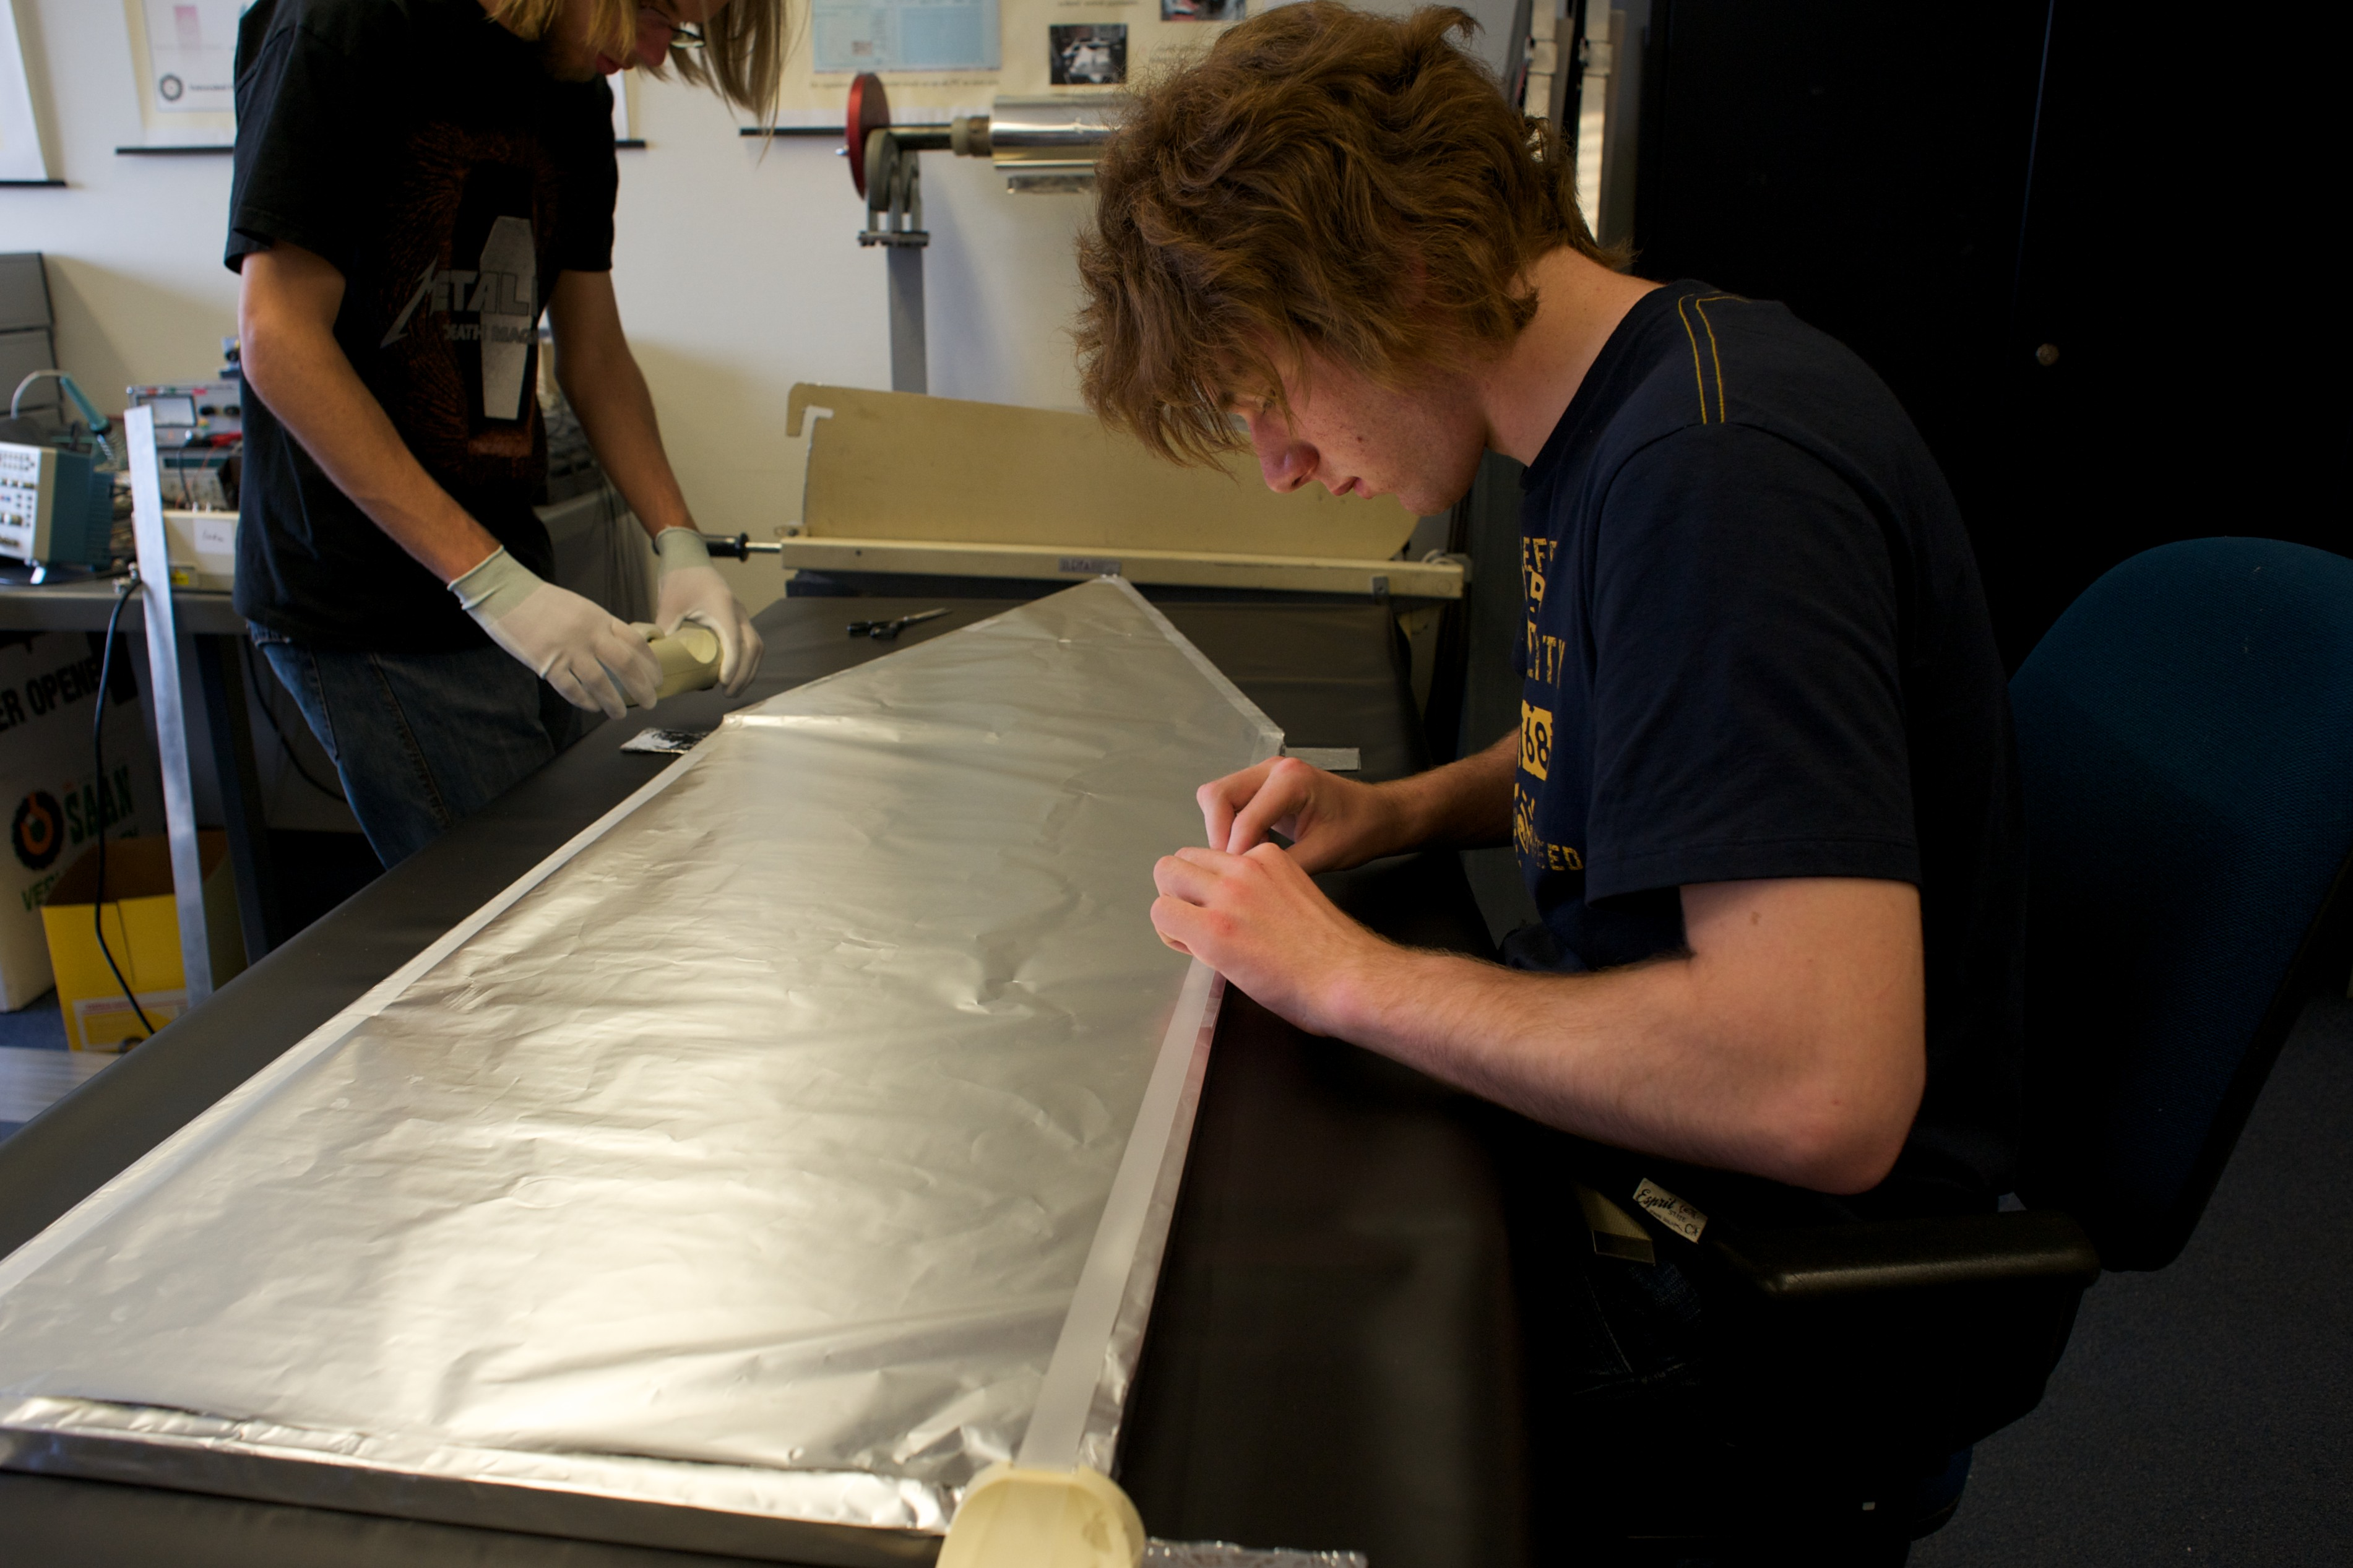
\includegraphics[width=0.6\textwidth]
                    {plots/cosmic-rays/ADL_100352}
    \caption{High-school students work on finishing a detector.}
    \label{fig:detector-bouw}
\end{figure}


\section{The work presented in this thesis}

The goal of the research presented in this thesis is the reconstruction of EAS detected with multiple detector stations from the \hisparc network. For reconstructions an understanding of the individual detectors and detector stations is required. Experiments and simulations have been performed to determine the accuracy and response of the various components.


\subsection{The \hisparc experiment
            (\crefrange{ch:experiment}{ch:cluster})}

In the next chapter the overall project is described, the layered structure of \hisparc is also explained. First at the overall project is described. The start and growth of the project are discussed and the organization structure explained.

Then the design an performance of the different scales is discussed. This starts with the individual detectors, the scintillators which detect the passing EAS particles. The construction of the detector has to be practical enough to be performed by high-school students. There are many interesting aspects concerning the signal strength and timing response of the detectors which is discussed in this part. As explained before/above a single detector is not enough to identify EAS from the background particles. Multiple detectors are combined to create a detector station which can pick out EAS from the background signals using a coincidence trigger. The readout, trigger logic, and timing of detector stations is explained. A single detector station is small enough to fit on a roof. Multiple detector stations are deployed in the \hisparc project. To combine the data accurate absolute timing and positioning is required for each station, a \gps module is used for this. Experiments to understand the accuracy of the \gps positioning and timing will be presented.


\subsection{Software infrastructure
            (\cref{ch:software,ch:data_processing})}

Without reliable software the \hisparc project could not exist. The detector stations are at locations which are sometimes far apart, each working autonomously. Though each stations has a person who is responsible for keeping that station working properly, they do not always have time to fix complex issues. Reliably working software is therefore important. The software that runs on the different \hisparc servers also needs to run without much maintenance. The analysis framework should also work as intended to prevent making each analysis a chore. A lot of effort has been put in extending the software while also increasing the reliability. In these chapters the different software packages are described, how they work together, and how the data flows through the different stages of the processing.


\subsection{Data analysis
            (\cref{ch:simulations,ch:analysis})}

EAS simulations are used to better understand shower development. Having gained knowledge about the detector, station, and cluster responses using theory, simulations, and experiments analysis algorithms are devised to perform calibration, data quality checks, and reconstruction of the detections. The calibration corrects for non-linear signal responses and timing offsets between different components. Data-quality cuts select data of good quality for the analysis. The reconstructions are improved to use more knowledge about shower development and the results from simulations. With these, information about the shower-core axis position and direction, and the shower size can be reconstructed.


\subsection{Science Park data analysis
            (\cref{ch:network,ch:conclusions})}

The analysis will be performed on a dataset of good data, selected from over \SI{10}{\year} of \hisparc data. The cuts that were done to end up with the final dataset are explained. The results will be compared to realistic simulations and other experiments. Finally the results are discussed.


\subsection{Coordinate systems and outreach
            (\cref{ch:coordinates,ch:outreach})}

At the end a summary of the different coordinate systems and units used by \hisparc and other relevant sources is discussed. And a more in-depth look at the outreach by \hisparc is presented.
